\documentclass[thesis=B,czech]{FITthesis}[2012/06/26]

\usepackage[utf8]{inputenc}

\usepackage{graphicx} %graphics files inclusion
\usepackage{amsmath} %advanced maths
\usepackage{amsthm}
\usepackage{dirtree} %directory tree visualisation
\usepackage{algorithm}
\usepackage{algpseudocode}
\usepackage{amssymb} %additional math symbols
\usepackage{bm}
\usepackage{epstopdf}
\usepackage{mathtools}
\usepackage{hyperref}
\usepackage{xr}
\usepackage{fancyvrb}
\usepackage{svg}


% % list of acronyms
% \usepackage[acronym,nonumberlist,toc,numberedsection=autolabel]{glossaries}
% \iflanguage{czech}{\renewcommand*{\acronymname}{Seznam pou{\v z}it{\' y}ch zkratek}}{}
% \makeglossaries

\newcommand{\tg}{\mathop{\mathrm{tg}}} %cesky tangens
\newcommand{\cotg}{\mathop{\mathrm{cotg}}} %cesky cotangens
\newcommand{\Break}{\State \textbf{break} } %prikaz break v algoritmech
\renewcommand{\algorithmicrequire}{\textbf{In:}}
\renewcommand{\algorithmicensure}{\textbf{Out:}}

\floatname{algorithm}{Algoritmus}

\theoremstyle{definition}
\newtheorem{definition}{Definice}

\department{Katedra teoretické informatiky}
\title{Heuristiky pro propagaci intervalů}
\authorGN{Jakub}
\authorFN{Kottnauer}
\authorWithDegrees{Jakub Kottnauer}
\supervisor{doc. Ing. Stefan Ratschan}
\acknowledgements{Děkuji doc. Ing. Stefanu Ratschanovi za vedení mé bakalářské práce a za ochotu poradit s~jakýmkoliv problémem při její tvorbě.}
\abstractCS{Omezující podmínka je relace mezi proměnnými omezující množiny hodnot, kterých mohou proměnné nabývat. Problém splnitelnosti omezujících podmínek (CSP) je problém, jehož řešení spočívá v~nalezení hodnot proměnných tak, aby byly splněny všechny zadané omezující podmínky. Hlavním cílem práce je otestování vlivu heuristik na~efektivitu řešení numerických CSP pomocí propagací intervalů. Součástí práce byl napsán řešič v~jazyce F\# implementující algoritmy HC3 a branch-and-prune s~podporou pro podmínky s~operacemi sčítání, odčítání a~násobení. Byly nalezeny podstatné parametry algoritmu ovlivňující jeho účinnost a~následně byly s~třinácti heuristikami provedeny výpočetní experimenty a~jejich výsledky porovnány. Výstup práce bude možno využít při rozvažování, kterou heuristiku použít při řešení soustav omezujících podmínek převeditelných na~podmínky s~výše uvedenými operacemi.}
\abstractEN{A constraint is a relation between variables which reduces the set of values that can be assigned to a variable. A constraint safisfaction problem (CSP) is the~problem of finding values for the variables in a given constraint that satisfy the constraint. The~main goal of this thesis is to test the influence of various heuristics on the efficiency of solving numerical CSP problems by interval propagation. A~solver written in the F\# language utilizing the HC3 algorithm and a branch-and-prune algorithm was created, important aspects of the HC3 algorithm influencing its efficiency were found and then experiments with thirteen different heuristics were performed. The results found in the thesis can be used when deciding which heuristic to use for solving constraint satisfaction problems.}
\placeForDeclarationOfAuthenticity{V~Praze}
\declarationOfAuthenticityOption{4} %volba Prohlášení (číslo 1-6)
\keywordsCS{propagace intervalů, algoritmus HC3, branch and prune, problém splnitelnosti, omezující podmínky, heuristiky, konzistenční techniky, funkcionální programování, FSharp}
\keywordsEN{interval propagation, HC3 algorithm, branch and prune, constraint satisfaction problem, constraints, heuristics, consistency, functional programming, FSharp}

\begin{document}

% \newacronym{CVUT}{{\v C}VUT}{{\v C}esk{\' e} vysok{\' e} u{\v c}en{\' i} technick{\' e} v Praze}
% \newacronym{FIT}{FIT}{Fakulta informa{\v c}n{\' i}ch technologi{\' i}}

\begin{introduction}
V mnoha oblastech lidské činnosti, ať už je to věda, podnikání, či sport, existují problémy, které kladou na svá řešení nějaká omezení. Takovým problémům se obecně říká problémy splnitelnosti omezujících podmínek (\emph{constraint satisfaction problems}). Omezující podmínky zde zužují množiny hodnot, kterých mohou nabývat proměnné vyskytující se v problému.

Tato bakalářská práce se zabývá speciálním typem CSP problémů, nazývaných numerické CSP problémy. Numerické CSP jsou takové problémy, které se dají popsat soustavou rovnic a~nerovnic a~jejichž proměnné nabývají hodnot z~reálných intervalů. Jedna z~možností, jak tyto problémy řešit, se nazývá \emph{propagace intervalů}. Tyto metody postupně zmenšují intervaly jednotlivých proměnných, až je dosaženo dostatečné přesnosti řešení. K~rozhodnutí, v~jakém pořadí zmenšovat intervaly a~zpracovávat omezující podmínky, pomáhají heuristiky.

Hlavním cílem této práce je otestovat vliv různých heuristik na efektivitu hledání řešení numerických CSP problémů, přičemž jednotlivé heuristiky budou porovnány na základě několika indikátorů naměřených v průběhu experimentů.

Práce je rozdělena do čtyř hlavních kapitol - v první kapitole je vysvětlena teorie nutná k implementaci řešiče, jenž byl vytvořen v rámci této práce. Druhá kapitola přehledně shrnuje cíle práce, kterých je dosaženo v posledních dvou kapitolách. Návrh řešiče, který dostal jméno HullSolver, je včetně použitých algoritmů popsán ve třetí kapitole. Poslední částí textu je popis experimentů provedených s programem a shrnutí výsledků.

Součástí dokumentu jsou také tři přílohy. V~příloze A jsou vysvětleny zkratky použité v~bakalářské práci. V~příloze B je uveden manuál k programu HullSolver a na závěr příloha C shrnuje obsah přiloženého CD.


\end{introduction}

\externaldocument{implementation.tex}

\chapter{Popis problematiky}
První část práce představuje úvod do teorie řešení problémů s omezujícími podmínkami. Nejprve jsou zde popsány základní typy těchto problémů a způsoby, jak je řešit. Poté následuje popis několika algoritmů a na závěr kapitoly jsou uvedeny heuristiky, které mohou pomoci zvýšit efektivitu řešení.


%%%%%%%%%%%%%%%%%%%%%%%%%%%%%%%%%%%%%%%
%%%%%%%%%%%%%%%%%%%%%%%%%%%%%%%%%%%%%%%
\section{Constraint programming}
\emph{Constraint programming} (či \emph{programování s~omezujícími podmínkami}) je jedním z~odvětví umělé inteligence pro řešení optimalizačních úloh, konkrétně problémů splnitelnosti omezujících podmínek (CSP problémy). Asociace ACM v~článku \cite{Wegner1996} označila toto téma jako jedno z~klíčových oblastí pro budoucí výzkum, neboť se problémy s~omezujícími podmínkami přirozeně vyskytují v~každodenním životě. Předností constraint programming je navíc to, že uživatel popíše problém k~vyřešení pouze deklarativně - nedá tedy počítači žádný postup k~řešení, jen zadá aktuální stav problému a specializovaný program (řešič) najde řešení (pokud existuje).

Typickým příkladem problému s~omezujícími podmínkami jsou různé hry, například sudoku. Jak ukazuje definice \ref{def:csp}, CSP se skládá z~proměnných, domén a omezujících podmínek. V~sudoku jsou proměnnými volná políčka na~hracím poli, z~nichž každá má svoji \emph{doménu} (množinu hodnot, kterých může teoreticky nabývat, v~tomto případě čísla 1 až 9). Omezujícími podmínkami jsou samotná pravidla hry - požadavek na~unikátnost číslice v~řádku, sloupci, resp. ve~čtverci. Pojmy \emph{doména} a \emph{omezující podmínka} přesněji vysvětlují definice č.~\ref{def:domain} a \ref{def:constraint} níže.

\begin{definition}[{\cite[s.~14]{rossi2006}}]
\label{def:csp}
\emph{CSP} (\emph{problém splnitelnosti omezujících podmínek}) je \\ trojice $(V, D, C)$, kde
\begin{itemize}
  \item $V$ je uspořádaná posloupnost proměnných,
  \item $D$ je uspořádaná posloupnost domén (viz definice č.~\ref{def:domain}) náležejících k~proměnným,
  \item $C$ je množina omezujících podmínek (viz definice č.~\ref{def:constraint}).
\end{itemize}
\end{definition}

Známý SAT problém\footnote{Boolean satisfiability problem} se také dá formulovat jako problém s~omezujícími podmínkami.

\subsection{Doména}
\begin{definition}[{\cite[s.~10]{Vu2005}}]
\label{def:domain}
\emph{Doména} (nebo také \emph{definiční obor}) proměnné je množina všech hodnot, kterých může proměnná nabývat.
\end{definition}

Doménou, jak ukazuje definice \ref{def:domain}, může být jakákoliv množina. Nejjednodušší jsou diskrétní konečné domény (podmnožiny přirozených čísel,\\ $\{red, green, blue \}$ při obarvování grafu, $\{ true, false \}$ u SAT problém, apod.). Diskrétní domény mohou být také nekonečné - v~takovém případě se může stát, že řešení nelze popsat jednoduše výčtem hodnot z~domén a je nutné jej popsat vztahem mezi proměnnými \cite[s.~139]{Russell:2003}.

V reálném světě se často vyskytují problémy se spojitými doménami, které mohou být reprezentovány pomocí intervalů (lineární programování je příkladem takového problému).


\subsection{Omezující podmínka}
\begin{definition}[{\cite[s.~11]{Vu2005}}]
\label{def:constraint}
\emph{Omezující podmínka} $c$ na~konečné posloupnosti proměnných $(x_1, \dots, x_n)$ s~doménami $(D_1, \dots, D_n)$, $n \in \boldsymbol{N}$, je podmnožina kartézského součinu $ D_1 \times \dots \times D_n $.
\end{definition}

Omezující podmínka dle definice \ref{def:constraint} je tedy relace mezi proměnnými a lze ji zapsat jako $c(x_1, \dots, x_n)$. Vzhledem k~tomu, že se jedná o~relaci, lze omezující podmínky rozdělit podle arity na~relace unární ($x \leq 1$), binární ($x = y$) a~více-ární ($x + y > z $) \cite[s.~139]{Russell:2003}.

V praktické části této práce budou omezující podmínky reprezentovány rovnicemi (jednoduchá rovnice $x = 0, x \in \boldsymbol{N}$ zjevně omezuje možné hodnoty proměnné $x$, jedná se tedy o omezující podmínku).

Omezující podmínka je \emph{redundantní} (nadbytečná) {\cite[s.~20]{Vu2005}}, nemá-li její odebrání z~CSP vliv na~řešení problému (v problému \\ $P = (V, D, C)$, kde $C = {c_1: x > y, c_2: x > y, c_3: y < x}$ jsou libovolné dvě podmínky redundantní).

Pro práci je důležité ještě jedno dělení omezujících podmínek, a to na~\emph{primitivní} a \emph{komplexní} podmínky (více viz \cite{kue12}). Omezující podmínka reprezentovaná rovnicí v~primitivním tvaru obsahuje maximálně jednu aritmetickou operaci (maximální arita podmínky je tedy rovna třem). Příkladem mohou být podmínky $x = y^2$ či $a = \sin b$). Toto rozdělení je důležité, protože algoritmus využitý v~praktické části umí pracovat pouze s~primitivními podmínkami a program je očekává na~vstupu. Před spuštěním programu je tedy nutné provést manuální rozklad podmínek a označit, které z~proměnných se vyskytovaly v~původních podmínkách. Takovým proměnným se říká \emph{dominantní}, ostatní jsou \emph{nedominantní}, nebo také \emph{pomocné} proměnné.

Rozdíl mezi ekvivalentními jednoduchými a komplexními podmínkami ukazují příklady č.~\ref{eq:complexConstraint} a \ref{eq:primitiveConstraint}. V~tomto příkladu jsou dominantními proměnnými $x$, $y$ a $z$.

\begin{equation} \label{eq:complexConstraint}
x + 2y + z = 1
\end{equation}

\begin{equation} \label{eq:primitiveConstraint}
v_1 = 2y \quad \wedge \quad v_2 = z - 1 \quad \wedge \quad v_3 = x + v_1 \quad \wedge \quad v_3 + v_2 = 0
\end{equation}





%%%%%%%%%%%%%%%%%%%%%%%%%%%%%%%%%%%%%%%
%%%%%%%%%%%%%%%%%%%%%%%%%%%%%%%%%%%%%%%
\section{Numerical constraint satisfaction problem}
\label{ch:ncsp}

Tato práce se zabývá řešením \emph{numerických CSP} (\emph{NCSP}, \emph{numerical CSP}), což je podmnožina CSP problémů, jejichž domény jsou spojité (nejčastěji jsou to intervaly) a které se dají reprezentovat soustavami rovnic či nerovnic. Rovnice nebo nerovnice vlastně kladou na~proměnné nějaká omezení a zmenšují tak množiny hodnot, kterých mohou nabývat \cite{rueherDependency}.

Domény proměnných v~NCSP problémech jsou reálné intervaly, a cílem řešiče je co nejvíce tyto intervaly zúžit (zúžení domény podle omezující podmínky se říká \emph{propagace omezující podmínky}, v případě NCSP se tento proces někdy nazývá \emph{propagace intervalů}), při zachování všech řešení soustavy rovnic tvořené omezujícími podmínkami. To ukazuje následující jednoduchý příklad \ref{eq:simpleConstraint}.

\begin{equation} \label{eq:simpleConstraint}
x^2 = 1\qquad x \in \boldsymbol{R}
\end{equation}

Nechť rovnice \ref{eq:simpleConstraint} představuje omezující podmínku a pro doménu $D_x$ proměnné $x$ platí $D_x = (-5;5)$. Všechna řešení této rovnice určitě leží v~intervalu $D_x$, ale také například v~$\langle -1;2)$, nikoliv však v~$(0;2)$ (tento interval obsahuje jen jedno ze dvou řešení). Metody řešení numerických CSP dokáží problém vyřešit nalezením minimálního intervalu obsahujícího všechna řešení, tj. $D_x' = \langle -1;1\rangle$. Nalezený interval vlastně tvoří jakési jednodimenzionální ohraničení všech možných řešení. V případě více než jedné proměnné je toto ohraničení tvořeno kartézských součinem intervalů a anglicky se nazývá \emph{box}.

Výhodou těchto problémů je fakt, že se dají (alespoň do počtu třech dominantních proměnných) snadno graficky vizualizovat. Domény proměnných představují jednotlivé osy, omezujícími podmínkami jsou funkce a boxy obalující řešení jsou skutečnými 2D či 3D \uv{krabicemi} okolo řešení.

Nebude-li řečeno jinak, bude se zbývající text právě věnovat především problematice numerických CSP.



%%%%%%%%%%%%%%%%%%%%%%%%%%%%%%%%%%%%%%%
%%%%%%%%%%%%%%%%%%%%%%%%%%%%%%%%%%%%%%%
\section{Intervalová aritmetika}
\label{ch:interval_arithmetic}
Intervalová aritmetika je rozšířením aritmetiky reálných čísel na~intervaly. Následující definice jsou převzaty~\cite{Moore:09}, s~výjimkou, že pro značení otevřených a~uzavřených intervalů je využita notace používaná v~české literatuře:

\begin{itemize}
    \item $\langle a;b \rangle \equiv \{x \in R | a \le x \le b \} $ - uzavřený interval
    \item $(a;b) \equiv \{ x \in R | a < x < b \}$ - otevřený interval
\end{itemize}

Pro sčítání, odčítání, násobení a dělení intervalů platí následující vztahy ($x = \langle a; b \rangle$ a $y = \langle c; d \rangle$ jsou intervaly a odpovídající vztahy platí i pro otevřené intervaly):

\begin{subequations}
\begin{align}
   x+y = \langle & a + c;  b + d \rangle\\
   x-y = \langle & a - c;  b - d \rangle\\
   \begin{split}x  \cdot y = \langle & min(ab, ad, bc, bd); \\ & max(ab, ad, bc, bd) \rangle \end{split}\\
   \frac{x}{y} = x & \cdot \frac{1}{y} \mbox{ pokud } 0 \notin y, \mbox{ kde } \frac{1}{y} \equiv \langle  \frac{1}{b}; \frac{1}{a} \rangle
\end{align}
\end{subequations}

Odčítání lze převést na~sčítání pomocí tohoto vztahu:

\begin{subequations}
\begin{align}
   -x = - \langle a;b \rangle = \langle -b; -a \rangle
\end{align}
\end{subequations}


Dalšími potřebnými operacemi jsou průnik a sjednocení:

\begin{subequations}
\begin{align}
   x \cap y = \{ & i \in R | i \in x \wedge i \in y \} \\
   x \cup y = \langle & min(a, c); max(b, d) \rangle
\end{align}
\end{subequations}

Jako \emph{intervalový obal} (\emph{interval hull}, značeno $H$) se označuje nejmenší interval \uv{obalující} podmnožinu reálných čísel. Například platí, že $H(\{2,5,8\}) = \langle 2; 8 \rangle$, $H((1;3) \cup (5;7)) = (1;7)$.

V souvislosti s intervaly je třeba zmínit ještě tzv.~\emph{dependency problem} (problém závislosti). To je situace, kdy se jeden interval vyskytuje na více místech výrazu a výsledný interval může být zbytečně široký. Dependency problem se projeví i na~velmi jednoduché rovnici $x - x = 0, x \in \langle 0;10 \rangle$. Na první pohled je správným řešením interval $\langle 0;0\rangle$, podle pravidel pro součet v~intervalové aritmetice bude ale výsledek $\langle 0;10 \rangle - \langle 0;10\rangle = \langle -10; 10 \rangle$.



%%%%%%%%%%%%%%%%%%%%%%%%%%%%%%%%%%%%%%%
%%%%%%%%%%%%%%%%%%%%%%%%%%%%%%%%%%%%%%%
\section{Řešení a splnitelnost CSP}
Přiřazení konkrétní hodnoty z~domény proměnné se nazývá \emph{ohodnocení} (\emph{label}). Přiřazuje-li ohodnocení hodnotu všem proměnným problému, jedná se o \emph{úplné ohodnocení} (\emph{compound label}). Tyto pojmy stačí k~definici řešení a splnitelnosti problému s~omezujícími podmínkami (definice \ref{def:solution}, resp. \ref{def:satisfiability}).

\begin{definition}[{\cite[s.~14]{rossi2006}}]
\label{def:solution}
\emph{Řešení} (\emph{solution}) CSP je takové úplné ohodnocení, pro které platí všechny omezující podmínky.
\end{definition}

\begin{definition}[{\cite[s.~14]{rossi2006}}]
\label{def:satisfiability}
CSP problém je \emph{splnitelný} (\emph{satisfiable}), existuje-li pro něj řešení.
\end{definition}

Podle charakteru problému někdy stačí nalézt jen jedno řešení, jindy je třeba nalézt všechna řešení, jindy je nutné najít optimální řešení.

Jak ale vůbec řešení problému probíhá? Nejprve je nutné zavést pojmy \emph{ekvivalence problémů} a \emph{redukce problému}. Dva CSP problémy jsou ekvivalentní, jsou-li nadefinované nad~stejnou posloupností proměnných a stejnou množinou omezujících podmínek a mají stejné množiny řešení \cite[s.~18]{Vu2005}. Například problémy

\begin{align*}
P_1 = ((x, y), (\{-1,0,1,2,3\}, \{1,2,3\}), \{x - y = 0\}) \\
P_2 = ((x, y), (\{1,2,3\}, \{1,2,3\}), \{x - y = 0\})
\end{align*}

jsou ekvivalentní a splnitelné. Na stejném příkladu lze demonstrovat i redukci problému. Redukce problému je transformace na~ekvivalentní a jednodušší CSP \cite[s.~23]{Vu2005}. Problém $P_2$ tak mohl vzniknout z~problému $P_1$ redukcí domény proměnné $x$, přičemž byly z~domény dané proměnné odebrány tzv.~\emph{nekonzistentní} hodnoty (hodnoty, pro které neexistuje řešení). Jak redukce může probíhat vysvětluje kapitola \ref{ch:narrowingHowWorks}, v~tuto chvíli ji stačí považovat za~černou skříňku, která na~vstupu přijme CSP a vrátí ekvivalentní zredukovaný problém.

\subsection{Branch-and-prune algoritmus}

Obecný postup pro řešení CSP, který je popsán algoritmem~\ref{alg:GeneralSolutionAlg} (převzatý z~\cite[s.~22]{Vu2005}) využívá k~nalezení řešení právě redukování problému.

\begin{algorithm}
\caption{Algoritmus Solve}
\label{alg:GeneralSolutionAlg}
\begin{algorithmic}[1]
\Require CSP problém $P = (V, D, C)$ k vyřešení.
\Ensure Zredukovaný problém $P$.
\Procedure{Solve}{$P$}
\State $continue \gets$ \verb|true|
\While{$continue$}
\State Zredukuj problém $P$ \label{alg:generalSolutionAlg:Reduction}
\If{not Happy}
\If{atomic}
\State $continue \gets $ \verb|false|
\Else
\State $P_1, P_2 \gets $\verb|Split| - rozděl problém a opakuj pro jednotlivé části
\State \verb|Solve|($P_1$)
\State \verb|Solve|($P_2$)
\EndIf
\Else
\State\Return $P$
\EndIf
\EndWhile
\State\Return $P$
\EndProcedure
\end{algorithmic}
\end{algorithm}

Algoritmus \verb|Solve| má tři důležité části - volání \verb|Happy| funkce, ověření \emph{atomicity} a rozdělení zredukovaného problému (\emph{splitting}). Spuštění algoritmu navíc často předchází předzpracování zadaného problému, jako například detekce a odstranění redundantních podmínek, nebo rozklad komplexních podmínek na~primitivní.

\begin{enumerate}
    \item Funkce \verb|Happy| ověřuje, jestli je program \uv{spokojený} s~aktuálním výsledkem a jestli může skončit. To může znamenat například to, jestli byl nalezen dostatečný počet řešení, nebo jestli bylo dokázáno, že žádné řešení neexistuje, apod.
    \item Ověření atomicity je kontrola, zda je zredukovaný problém již dostatečně malý, aby byl přijat jako řešení. Pro určení velikosti problému lze využít několik metrik, v~případě NCSP se nejčastěji používá měření velikosti domén dominantních proměnných a to buďto absolutní, nebo relativní vzhledem k~původní velikosti (například požadavek na~zmenšení domény na~tisícinu původní velikosti).
    \item Nebyl-li problém dostatečně zmenšen, dojde k~jeho rozdělení na~více částí (resp. na~několik menších CSP). To v~praxi nejčastěji znamená, že dojde k~rozdělení domén podle nějakého pravidla, kterých lze vymyslet poměrně velké množství: u~CSP s~diskrétními doménami je jedno z~možných rozdělení takové, kdy se z~domény nějaké proměnné vyjme jedna hodnota a ta se použije u problému $P_1$ a zbytek hodnot z~domény se použije u problému $P_2$. U problému $P_1$ pak lze velmi rychle rozhodnout, zda patří do~řešení, nebo ne. U numerických CSP problémů je nejjednodušší nějakým způsobem rozdělit jeden či více intervalů (domén). V~programu vytvořeném pro tuto práci je při každém rozdělení rozpůlena doména jedné proměnné, která je vybrána metodou \emph{round-robin}. To znamená, že jsou voleny jedna po~druhé, tak jak jdou za sebou v~definici problému zadaného uživatelem.
\end{enumerate}

Ohledně rozdělení problému na~menší části se možná nabízí otázka, proč je to vůbec potřeba, když redukce problému (řádek č.~\ref{alg:generalSolutionAlg:Reduction} v~pseudokódu) by měla být schopná odstranit nekonzistentní hodnoty z~domén. V~některých typech problému (a je to případ i NCSP problémů řešených zde) a v~závislosti na~použitém algoritmu se může stát, že se algoritmus zastaví na~krajních hodnotách domény. Obrázek č.~\ref{img:solving} znázorňuje průběh řešení NCSP problému s~využitím splittingu.

Červená a modrá křivka jsou omezující podmínky (soustava dvou rovnic) a zelený rámeček okolo nich v~bodu 1 je box tvořený doménami proměnných. Řešení problému se pochopitelně nalézá v~průsečících obou křivek, algoritmus ale při prvním průchodu dokáže box zmenšit maximálně tak, jak je ukázáno v~bodu 2. Následně dojde k~rozpůlení jedné z~domén a algoritmus se znovu spustí pro obě poloviny, které se již podaří maximálně zredukovat.

\begin{figure}
\centering
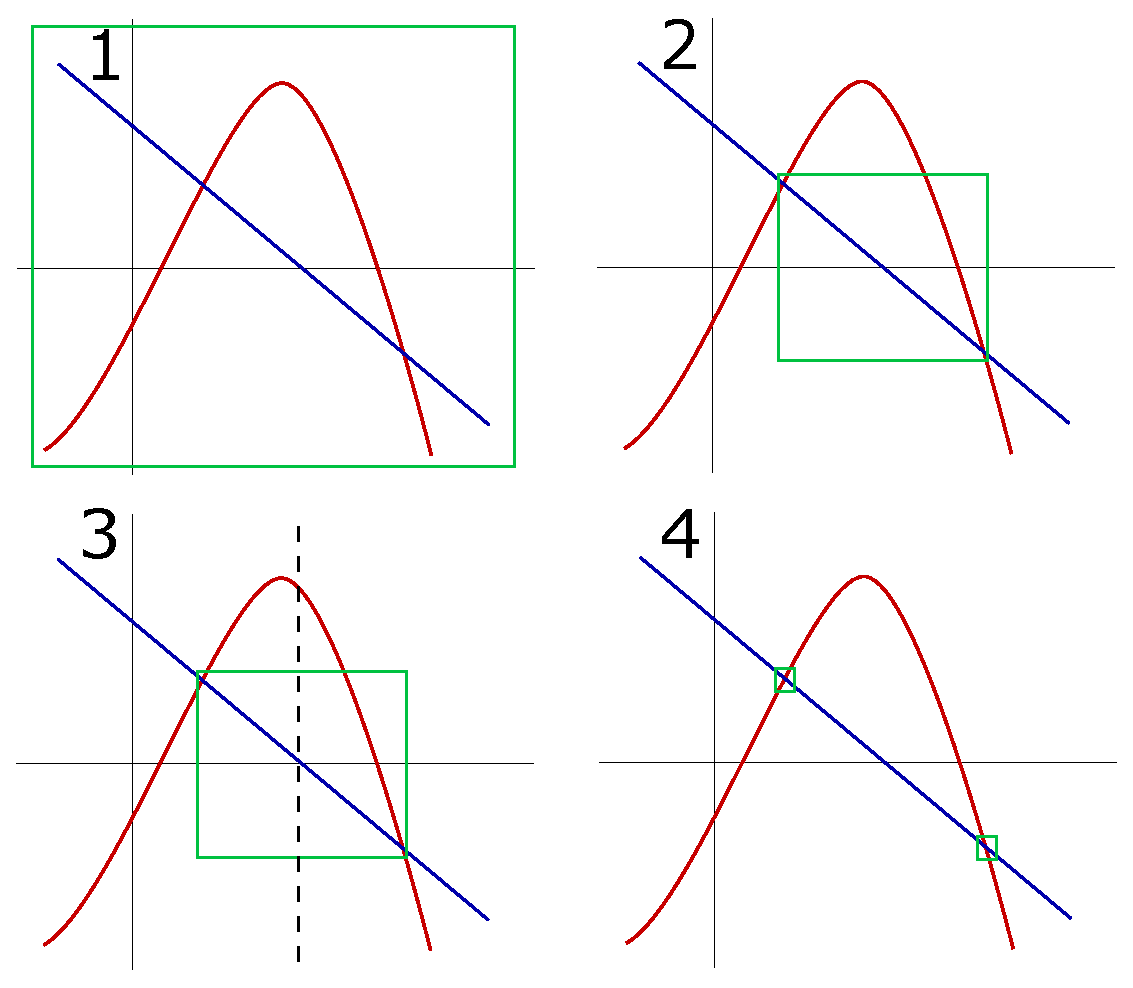
\includegraphics[scale=.68]{img/solving.eps}
\caption{Průběh algoritmu Solve s rozdělováním na menší problémy}
\label{img:solving}
\end{figure}

Algoritmům tohoto typu se říká \emph{branch-and-prune} algoritmy, což je volně přeložitelné jako \uv{větvení a odřezávání větví} - řešení se při zavolání \verb|Split| rozdělí na~několik větví, z~nichž ty, které nevedou k~řešení, budou odřezány.

Jak bude vidět v implementační části, řešič vytvoření v~této práci používá podobný algoritmus, viz algoritmus~\ref{BranchPrune} na straně~\pageref{BranchPrune}.







\subsection{Propagace omezujících podmínek se sčítáním a násobením}
\label{ch:narrowingHowWorks}
Teoretický základ pro propagaci omezujících podmínek se sčítáním, násobením a několika dalšími operaci položil John G. Cleary v~roce 1987 ve~svém článku \emph{Logical Arithmetic}~\cite{cleary87}. Tabulka~\ref{narrowingTable} ukazuje příklad (převzatý z~\cite{cleary87}) redukce domény pro omezující podmínku ve~tvaru $z = x + y$. Pro zúžení domény jedné proměnné stačí proměnnou vyjádřit z~rovnice a provést průnik její domény s~intervalem vzniklým z~výrazu na~druhé straně rovnice. Například pro zredukovanou doménu $D_z'$ proměnné $z$ platí $D_z' = D_z \cap (D_x + D_y)$.



\begin{table}
\centering
\begin{tabular}{|l|l|l|l|}
\hline
 Počáteční domény & $x \in \langle 0;2 \rangle$ & $y \in \langle 1;3 \rangle$ & $z \in \langle 4;6 \rangle$  \\ \hline
 $z = x+y$  &  & &  $\langle 1;5 \rangle$  \\ \hline
 $y = z-x$  & & $\langle 2;6 \rangle$  &  \\ \hline
 $x = z-y$  & $\langle 1;5 \rangle$  &  &  \\ \hline
 Nové domény & $x \in \langle 1;2 \rangle$ & $y \in \langle 2;3 \rangle$ & $z \in \langle 4;5 \rangle$ \\ \hline
\end{tabular}
\caption{Příklad redukce domén proměnných v podmínce $z = x + y$}
\label{narrowingTable}
\end{table}


Propagace podmínek s~násobením lze provést podobně, s~jednou komplikací, kterou odhalí následující příklad. Omezující podmínku $y = z \cdot x; x \in \langle -2;3 \rangle; y \in \langle -\infty ; \infty \rangle; z \in \langle 1;1 \rangle $ lze chápat jako rovnici $ y = \frac{1}{x}$ a je vidět, že žádný z~intervalů není možné přímo zmenšit a to i přesto, že doména proměnné $y$ obsahuje podmnožinu hodnot, kterých nemůže nabývat ($ \langle -\frac{1}{2};\frac{1}{3} \rangle $). Tento problém lze vyřešit pomocí funkce \verb|Split| z~algoritmu~\ref{alg:GeneralSolutionAlg}. O operacích, které trpí stejným problém se říká \emph{intervalově konvexní}, zatímco operace jako sčítání jsou \emph{intervalově konkávní} \cite{cleary87}.

Samotný algoritmus pro propagaci omezující podmínky s násobením je poměrně dlouhý, a proto zde nebude uveden. Jeho délka je způsobena tím, že se rozvětvuje podle toho, které meze intervalů jsou větší či menší než nula. Rozvětvení je uvedeno v~tabulce v~článku \cite{hickeyImplementation}.

V několika jednoduchých krocích (a to pouze s~využitím pravidel intervalové aritmetiky) se tak povedlo zúžit domény všech proměnných a vztahy mezi proměnnými přitom stále platí. Existuje důkaz (viz \cite{cleary87}), že je zbytečné snažit se volat zužovací funkci na~omezující podmínku vícekrát okamžitě po~sobě, domény se vždy maximálně zmenší již při prvním spuštění. V~případě, kdy se proměnná vyskytuje ve~více než jedné omezující podmínce ale může nastat situace, kdy následkem zúžení domény podle jedné podmínky dojde k~rozšíření domény vzhledem k~jiné podmínce a tak může být potřeba znovu zúžit tuto doménu podle již použité podmínky.





%%%%%%%%%%%%%%%%%%%%%%%%%%%%%%%%%%%%%%%
%%%%%%%%%%%%%%%%%%%%%%%%%%%%%%%%%%%%%%%
\section{Konzistenční techniky a algoritmy}
Konzistenční techniky slouží k~rychlému odebrání nekonzistentních (neplatných) hodnot z~domén proměnných a jejich cílem je dostat CSP do \emph{konzistentního stavu}, kdy domény neobsahují žádné nekonzistentní hodnoty. V~této kapitole je popsáno několik základních technik využitelných především pro nenumerické CSP a je ukázán přechod od nich na~techniku zvanou \emph{hull consistency}, používanou pro NCSP, která je pro tuto práci nejdůležitější, protože právě ona je využita v~praktické části.

\subsection{Node consistency}

\begin{definition}[{\cite[s.~16]{rossi2006}}]
\label{def:nodeConsistency}
Proměnná je \emph{node konzistentní}, je-li každá hodnota z~její domény konzistentní pro všechny unární omezující podmínky.
\end{definition}

Nejjednodušší konzistenční technikou je \emph{node consistency} \cite{bartakGuide} (viz algoritmus č.~\ref{NCAlgorithm}), pomocí které se dá velmi snadno (alespoň u diskrétních domén) dosáhnout konzistence tím, že program prochází hodnoty z~domény jednu po~druhé a pro každou hodnotu ověřuje, zda má pro všechny unární omezující podmínky smysl. Pokud nemá, je odebrána.


\begin{algorithm}
\caption{Algoritmus NC}
\label{NCAlgorithm}
\begin{algorithmic}[1]
\Require CSP problém $P = (V, D, C)$ k vyřešení.
\Ensure CSP bez nekonzistentních hodnot (podle node consistency) v doménách.
\Procedure{NC3}{$V, D, C$}
\For{každou proměnnou $v \in V$}
\For{každou hodnotu $x$ v doméně proměnné $v$}
\For{každou omezující podmínku $c \in C$}
\If{$x$ nesplňuje podmínku $c$}
\State Odstraň $x$ z domény.
\EndIf
\EndFor
\EndFor
\EndFor
\EndProcedure
\end{algorithmic}
\end{algorithm}


\subsection{Arc consistency}

\begin{definition}[{\cite[s.~16]{rossi2006}}]
\label{def:arcConsistency}
Proměnné $x$ a $y$ jsou \emph{arc konzistentní}, existuje-li pro každou hodnotu z~domény proměnné $x$ hodnota z~domény proměnné $y$ tak, že všechny omezující podmínky mezi těmito dvěma proměnnými platí.
\end{definition}

Diskrétní CSP problém se dá představit jako orientovaný graf (omezující podmínka je relace mezi proměnnými). Název této konzistenční techniky pochází z~jednoho anglických názvů pro hranu (\uv{arc}).

Pro dosažení tohoto typu konzistence existuje několik algoritmů, z~nichž poměrně jednoduchý a zároveň efektivní je algoritmus AC3 \cite{bartakGuide}. AC3 postupuje tak, že pro každou dvojici proměnných $(x, y)$ odstraní z~domény proměnné $x$ všechny hodnoty nekonzistentní s~hodnotami z domény proměnné $y$. Algoritmus si udržuje seznam hran ke~zkontrolování a při odebrání alespoň jedné hodnoty z~domény proměnné $x$ jsou do zmíněného seznamu přidány všechny hrany směřující do uzlu reprezentujícího proměnnou $x$.






\subsection{Hull consistency}

Jak node consistency, tak i arc consistency, se hodí spíše pro CSP s~diskrétními doménami, protože vždy pracují s~konkrétními hodnotami. V~případě spojitých domén je výhodnější nalézt obal, který zaručeně pokrývá všechny konzistentní hodnoty, i za cenu toho, že některé hodnoty v~něm budou nadbytečné. Takto funguje právě hull consistency.

\begin{definition}[{\cite[s.~572]{rossi2006}}]
\label{def:hullConsistency}
Omezující podmínka je \emph{hull konzistentní}, pokud kartézský součin domény proměnných z~dané podmínky tvoří intervalový obal všech řešení splňující danou podmínku. CSP problém $P$ je hull konzistentní, jsou-li všechny jeho omezující podmínky hull konzistentní.
\end{definition}

Jsou známy dva základní algoritmy k~dosažení hull consistency - \emph{HC3} a~\emph{HC4}.

Tyto algoritmy jsou vhodné především v~případě, kdy se jedna proměnná nevyskytuje v~mnoha podmínkách najednou. Pokud tomu tak je, může nastat situace podobná dependency problemu popsanému v kapitole~\ref{ch:interval_arithmetic}. Existují jiné konzistenční techniky (např. \emph{box consistency}), které si s~tímto problémem poradí \cite{rueherDependency}.

Tyto techniky se dají dále kombinovat například s~\emph{branch-and-prune} algoritmy, které umožňují rekurzivně rozpůlit nalezený box a tyto poloviční boxy dále zmenšovat pomocí HC algoritmů. Je tak možné získat několik menších boxů, které budou zahrnovat méně nadbytečných hodnot.

\subsubsection{HC3}
Algoritmus HC3 byl navržen jako první z~algoritmů pro propagaci intervalů v~roce 1997 v~článku \cite{Benhamou97applyinginterval}, autoři ho tehdy nazvali jednoduše jako \uv{A narrowing algorithm}. Název HC3 byl vytvořen později v~článku \cite{Benhamou99revisinghull} (tento název byl vybrán pro podobnost s~algoritmem AC3 používaným pro dosažení arc consistency), kde byl uveden i pokročilejší algoritmus HC4, který na rozdíl od HC3 nevyžaduje vstupní podmínky rozložené do primitivního tvaru.
 
Původní algoritmus HC3 navržený v~článku \cite{Benhamou97applyinginterval} je uveden v~pseudokódu č.~\ref{HC3Algorithm}, tvar algoritmu reálně použitý v~této práci je uveden v~implementační části.

\begin{algorithm}
\caption{Algoritmus HC3}
\label{HC3Algorithm}
\begin{algorithmic}[1]
\Require CSP problém $P = (V, D, C)$ k vyřešení.
\Ensure Informace o hull nekonzistenci, nebo zmenšený problém $P$.
\Procedure{HC3}{$V, D, C$}
\State $Q \gets C$
\While{$Q \neq \emptyset$ }
\State Vyber podmínku $c$ z $Q$.
\State $Q \gets Q \setminus \{ c \}$
\State $\{ x_1, ..., x_n\} \gets $ proměnné z $V$ vyskytující se v $c$.

\For{každé $x_i \in \{x_1, ..., x_n \} $}
\State $D_i' \gets $ zredukuj doménu $D_i$ proměnné $x_i$ podle podmínky $c$.
\If{$D_i' = \emptyset$}
\State \Return CSP je nekonzistentní.
\EndIf
\If{$D_i' \neq D_i $}
\State $D_i \gets D_i'$
\State Přidej do $Q$ podmínku $c$ a všechny další podmínky z $C$, které obsahují proměnnou $x_i$.
\EndIf
\EndFor
\EndWhile
\State \Return $P$
\EndProcedure
\end{algorithmic}
\end{algorithm}


\subsubsection{HC4}
Výhoda algoritmu HC4 oproti HC3 spočívá ve~faktu, že umí přímo pracovat s~komplexními podmínkami a není tak potřeba jejich rozklad, což ve~výsledku zkracuje i dobu běhu algoritmu \cite{Benhamou99revisinghull}. Nevýhodou je ovšem mnohem složitější implementace, která se skládá ze dvou fází: dopředného průchodu (\emph{ForwardEvaluation}) a zpětného průchodu (\emph{BackwardEvaluation}).

Celý algoritmus funguje tak, že prochází syntaktický strom výrazu a při dopředném průchodu od listů ke kořeni odhaduje domény rodičovských uzlů podle domén synů (s pomocí intervalové aritmetiky). Průběh pro omezující podmínku $2x = z - y^2$ s~doménami $D_x = \langle 0;20\rangle$, $D_y = \langle -10;10\rangle$ a $D_z = \langle 0;16\rangle$ ukazuje obrázek č.~\ref{img:forwardPropag}.

\begin{figure}
\centering
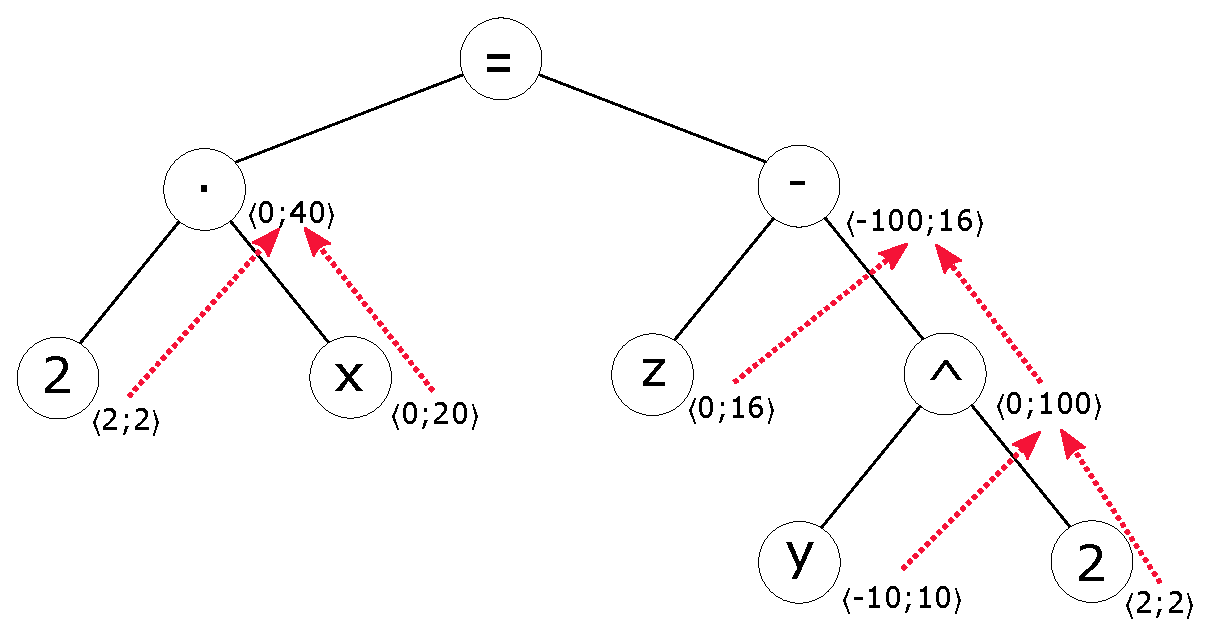
\includegraphics[scale=.65]{img/forwardPropag.eps}
\caption{Dopředný průchod u algoritmu HC4}
\label{img:forwardPropag}
\end{figure}

Při zpětném průchodu (obrázek č.~\ref{img:backwardPropag}) od kořene k~listům se pak zpřesňuje výsledná doména - podle rodičovského uzlu se zúží domény synů. Algoritmus u~kořene provede stromu z~předchozího příkladu provede průnik (kvůli rovnosti v~kořeni stromu) domén obou synů ($\langle 0;40\rangle \cap \langle -100;16\rangle$), které byly vypočteny při dopředném průchodu. Tímto je kořen zpracován a zpětný průchod se může spustit rekurzivně pro oba podstromy. V~případě levého podstromu je novým kořenem uzel s~operací násobení a doménou $\langle 0;16 \rangle$. Nyní je již snadné zúžit doménu proměnné $x$ na~její finální hodnotu, $\langle 0;8 \rangle$. Stejným postupem se podaří zúžit i domény proměnných $y$ a $z$ na~$\langle -4;4 \rangle$, resp. $\langle 0;16 \rangle$.

\begin{figure}
\centering
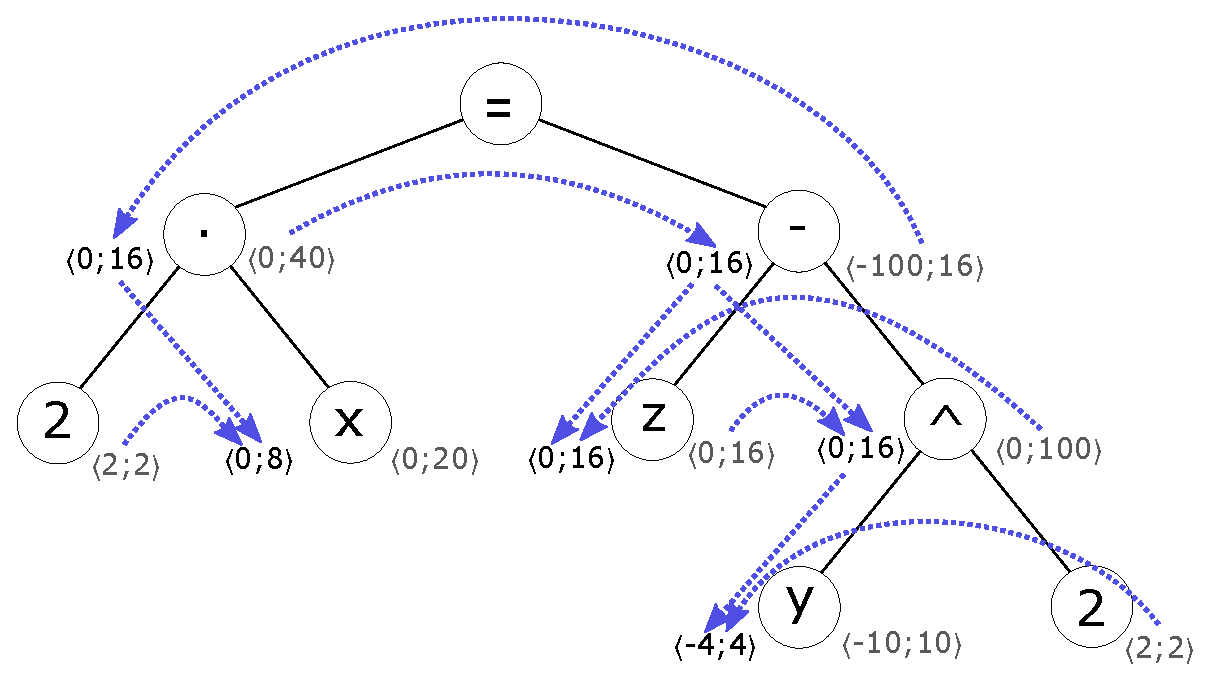
\includegraphics[scale=.65]{img/backwardPropag.eps}
\caption{Zpětný průchod u algoritmu HC4}
\label{img:backwardPropag}
\end{figure}







%%%%%%%%%%%%%%%%%%%%%%%%%%%%%%%%%%%%%%%
%%%%%%%%%%%%%%%%%%%%%%%%%%%%%%%%%%%%%%%
\section{Heuristiky}
Heuristiky při řešení problémů s~omezujícími podmínkami pomáhají rozhodnout, podle jaké omezující podmínky zužovat domény a v~jakém pořadí je zužovat. Jsou stále předmětem výzkumu a neexistuje žádný důkaz, který by prokazoval nějakou heuristiku lepší, než všechny ostatní. 

\subsection{Typy heuristik}
Heuristiky pro řešení NCSP se dají rozdělit do následujících dvou skupin \cite{feiten10}:

\begin{itemize}
  \item Heuristiky rozhodující podle statických (neměnných) vlastností proměnných, například počtu jejich výskytů, nebo aritmetických operací, kterých se účastní.
  \item Heuristiky rozhodující podle domén proměnných - zúžit širokou doménu může být výhodnější než dále zužovat malou doménu. Tyto vlastnosti jsou dynamické, tj. mění se během průběhu algoritmu.
\end{itemize}


Jedním z~cílů této práce je otestovat vliv heuristik na~efektivitu řešení různých problémů a v~následujících podkapitolách je uvedeno několik nápadů na~možné heuristiky (část jich je převzata z~\cite{feiten10}), z~nichž některé jsou využity v~praktické části. Seznam není vyčerpávající, jistě jich lze vymyslet o~mnoho více. Konkrétní heuristiky využité v~této práci jsou uvedeny v~praktické části v~kapitole~\ref{ch:usedHeuristics}. Všechny heuristiky uvedené v~této práci se vztahují k~algoritmu HC3.

\subsubsection{Statické parametry}

Heuristiky rozhodující podle statických parametrů se mohou řídit podle:

\begin{itemize}
  \item dominance či nedominance proměnné,
  \item vstupní množiny podmínek:
        \subitem počtu podmínek, ve~kterých se proměnná vyskytuje,
        \subitem počtu dominantních proměnných v~podmínce,
        \subitem operace použité v~omezující podmínce (sčítání/násobení).
\end{itemize}

\subsubsection{Dynamické parametry}

Heuristiky využívající dynamické parametry mohou brát ohled na:

\begin{itemize}
    \item intervaly:
        \subitem jejich velikost,
        \subitem zda pokrývají kladné i záporné hodnoty,
    \item zda se omezující podmínka již použila ke zredukování domény.
\end{itemize}

U dynamických parametrů se může vyplatit ukládat posloupnost změn hodnot tak, jak se měnily během běhu programu. V~praxi se ale při rozhodování nepoužívá celá posloupnost, jen její část. Následující parametry pracují s~historií změn:

\begin{itemize}
  \item poměr velikosti domény či problému k~původní velikosti,
  \item poměr aktuální velikosti k~velikosti v~minulém průběhu smyčky,
  \item číslo průběhu smyčky, kdy se naposledy používala podmínka ke zredukování domény.
\end{itemize}


%%%%%%%%%%%%%%%%%%%%%%%%%%%%%%%%%%%%%%%
%%%%%%%%%%%%%%%%%%%%%%%%%%%%%%%%%%%%%%%
\section{Charakteristiky problémových instancí pro algoritmus HC3}

Problémy k~řešení mají některé vlastnosti, které přispívají k~nižší efektivitě při řešení. Jsou jimi například:


\begin{itemize}
  \item výskyt jedné proměnné ve~více omezujících podmínkách,
  \item počáteční velikosti domén,
  \item počet proměnných,
  \item počet omezujících podmínek.
\end{itemize}

V~praktické části je ověřen vliv uvedených vlastností.


\chapter{Cíl práce}
Cílem práce je vytvoření jednoduchého řešiče pro NCSP ve funkcionálním jazyce \texttt{F\#} komunikujícího s uživatel přes příkazovou řádku, nalezení částí algoritmu, které ovlivňují jeho účinnost a rychlost, implementace heuristik nalezených v literatuře či vlastních nápadů (v jakém pořadí je nejlepší domény zužovat, atp.) a experimentálně porovnat účinnost jednotlivých heuristik.
\externaldocument{theory.tex}



\chapter{Implementace}
Jako součást bakalářské práce byl vytvořen řešič numerických CSP s~názvem \emph{HullSolver}, který jako jediný volně dostupný řešič umožňuje porovnávat efektivitu použitých heuristik. Zdrojové kódy jsou dostupné pod licencí GNU GPL na~serveru GitHub\footnote{\url{https://github.com/jakubkottnauer/hull-solver}}, případně jsou k nalezení i na~přiloženém CD. Manuál popisující kompilaci, spuštění a použití programu je uveden na~konci práce v~příloze \ref{hullSolverManual}.

Tato část práce nejprve popisuje použité technologie a~algoritmy v~programu HullSolver, následně se věnuje popisu architektury programu a na~závěr uvádí několik existujících řešení, které řeší podobné problémy.


\section{Použité technologie}
Jako jazyk pro implementaci byl zvolen funkcionální jazyk \texttt{F\#} (čteno jako F Sharp) běžící na~platformě .NET, který se v~posledních letech stal velmi populární pro vědecké využití. Tento jazyk byl poprvé uveden v~roce 2005 společností Microsoft, v~roce 2013 byla ale založena nezisková společnost \texttt{F\#} Software Foundation, která má na~starosti jeho další vývoj. Od~té doby se z~jazyka stal open-source a díky projektu Mono je možné aplikace napsané v~\texttt{F\#} spouštět i na~jiných platformách, než pouze na~Microsoft Windows.

\section{Algoritmy}

S~vedoucím práce bylo dohodnuto, že řešič bude podporovat omezující podmínky s~operacemi sčítání, odčítání a násobení.

Řešení vstupních problémů probíhá s~využitím algoritmu HC3 s~malou úpravou pro pestřejší možnosti využití heuristik. Zatímco originální algoritmus vždy vybere z~množiny podmínek jednu náhodnou a zredukuje domény všech proměnných v~ní obsažených, upravený algoritmus na vstupu přijímá množinu všech dvojic $(c, x)$ (kde $c$ je omezující podmínka definovaná nad proměnnou $x$) a z~této množiny heuristicky vybírá jednu dvojici. Následně podle podmínky $c$ zúží doménu proměnné $x$. Omezující podmínka $c$ se tedy na~vstupu objeví tolikrát, nad~kolika proměnnými je nadefinována - v~případě programu HullSolver vždy právě třikrát, neboť program podporuje pouze ternární omezující podmínky. Algoritmus~\ref{HC3AlgorithmAltered} uvádí pseudokód takto upraveného algoritmu HC3.

\begin{algorithm}
\caption{Upravený algoritmus HC3}
\label{HC3AlgorithmAltered}
\begin{algorithmic}[1]
\Require Seznam $P$ dvojic $(c, x)$, kde $c$ je omezující podmínka definovaná nad proměnnou $x$, a množina domén $D$ z CSP.
\Ensure Informace o nekonzistenci, nebo zmenšený problém $P$.
\Procedure{HC3}{$P, D$}
\State $Q \gets P$
\While{$Q \neq \emptyset$ }
\State Pomocí heuristiky vyber z $Q$ pár $p = (c, x)$.
\State $Q \gets Q \setminus \left\{ p \right\}$
\State $D_x' \gets$ Zredukuj doménu $D_x \in D$ proměnné $x \in p$ podle $c$.
\If{$D_x' = \emptyset $}
\State \Return CSP je nekonzistentní.
\EndIf
\If{$D_x \neq D_x'$}
\State $D_x \gets D_x'$
\State Přidej do $Q$ pár $p$ a všechny další páry z $P$, které obsahují $x$.
\EndIf
\EndWhile
\State \Return $P$
\EndProcedure
\end{algorithmic}
\end{algorithm}

Na řádku č.~7 v algoritmu \ref{HC3AlgorithmAltered} jsou pro rovnost porovnávány dvě domény. Vzhledem k tomu, že jsou zde domény tvořeny reálnými intervaly, nemusí být jejich meze celá čísla a v počítači tak nebudou uložena přesně (v programu je pro reprezentaci mezí využit 64-bitový typ \verb|double|). Rovnost je v programu ověřována nepřesně, jak ukazuje následující kód (jako \verb|ZERO_EPSILON| je použita hodnota $10^{-30}$):

\begin{Verbatim}[samepage=true]
member this.EqualTo y =
  abs(this.a - y.a) < ZERO_EPSILON 
  && abs(this.b - y.b) < ZERO_EPSILON
\end{Verbatim}

Nad algoritmem HC3 je postaven jednoduchý branch-and-prune algoritmus (viz Algoritmus \ref{BranchPrune}), který zároveň tvoří hlavní funkci řešiče. Tento algoritmus přibližně kopíruje strukturu algoritmu~\ref{alg:GeneralSolutionAlg} (str.~\pageref{alg:GeneralSolutionAlg}), jen je zde využit rekurzivní zápis. Při spuštění je mu předána množina dvojic omezujících podmínek a proměnných v~nich obsažených.

\begin{algorithm}
\caption{Rekurzivní algoritmus Solve}
\label{BranchPrune}
\begin{algorithmic}[1]
\Require Seznam $P$ dvojic $(c, x)$, kde $c$ je omezující podmínka definovaná nad proměnnou $x$, a množina domén $D$ z CSP.
\Ensure Seznam nalezených boxů.
\Procedure{Solve}{$P, D$}
\If{Problém není dostatečně malý}
\State $P' \gets HC3(P)$
\State $(P_1, P_2) \gets $ rozděl box tvořený doménami dominantních proměnných z $D$ na poloviny.
\State Solve($P_1$)
\State Solve($P_2$)
\Else
\State Vypiš/ulož box tvořený proměnnými z $P$ jako jeden z výsledků.
\EndIf
\EndProcedure
\end{algorithmic}
\end{algorithm}

V použité variantě algoritmu \verb|Solve| je kontrolováno, zda je problém již dostatečně zmenšen. V programu se konkrétně kontroluje, jestli se již podařilo domény všech dominantních proměnných dostatečně zúžit vzhledem k původní velikosti. Jako koeficient pro porovnání se využívá parametr \verb|eps|, který je specifikován uživatelem při spuštění řešiče přepínačem \verb|-p| (viz manuál).

\begin{Verbatim}[samepage=true]
member this.AllFraction eps =
  dominantVariables 
  |> List.forall(fun v -> 
    (v.Domain.Length / v.OriginalDomain.Length) < eps)
\end{Verbatim}


Druhým prvkem algoritmu \verb|Solve|, jehož implementace je potřeba upřesnit, je rozpůlení boxu na~řádku č.~4. Box, jak je popsáno v kapitole \ref{ch:ncsp}, ohraničuje řešení a je tvořen doménami proměnných z~CSP. Algoritmus box rozpůlí tím, že rozpůlí doménu jedné dominantní proměnné. Ve~vstupním souboru uživatel označí dominantní proměnné a algoritmus je půlí metodou round-robin ve~stejném pořadí, jako jsou zapsány ve~vstupním souboru (při rozpůlení poslední dominantní proměnné přeskočí opět na~první).


\section{Architektura}
Celý program se skládá ze čtyř souborů - \verb|DomainTypes.fs|, \verb|Heuristics.fs|, \verb|Solver.fs|, \verb|Program.fs|. Při kompilování programu napsaného v~\texttt{F\#} záleží na~pořadí souborů a v~tomto případě jsou soubory zpracovávany v~tomto pořadí. Braním ohledu na~pořadí souborů kompilátor zabraňuje tvorbě kruhových závislostí mezi částmi programu, protože soubor později ve frontě může využívat pouze typy z~již zpracovaného souboru. Kód se tak stává modulárnější a přehlednější, protože přirozeně dochází ke striktnímu oddělení \uv{high-level} částí programů od \uv{low-level} částí.

Dalším důsledkem je odlišná organizace kódu v~podobných jazycích jako \texttt{F\#} od klasických procedurálních či objektově orientovaných jazyků. V~\texttt{F\#} se typicky nevytváří samostatný soubor pro každý typ (typ přibližně odpovídá třídě z~objektově orientovaného programování), ale všechny typy se shlukují do jednoho modulu často nazývaného \verb|DomainTypes|. V~případě HullSolveru jsou doménovými typy \verb|Interval|, \verb|Variable|, \verb|Constraint|, \verb|Problem| a~\verb|Heuristic|, z~nichž poslední se pro~přehlednost nachází v~samostatném souboru \verb|Heuristics.fs|.

Zatímco první dva soubory obsahují především deklarace typů a definují jejich funkce, soubor \verb|Solver.fs| tvoří hlavní výpočetní jádro programu - zde jsou implementace branch-and-prune algoritmu a algoritmu HC3. Posledním souborem je \verb|Program.fs|, který se už stará jen o ošetření a zpracování vstupu a spouští řešící algoritmy.

\section{Výstup programu a indikátory}
\label{ch:indicators}
V průběhu řešení problémů je sledováno několik tzv. indikátorů. To jsou různé zajímavé metriky, pomocí kterých se dá následně porovnat efektivita heuristik. Kromě času běhu algoritmu (který je ale spíše pouze ilustrativní, protože se může měnit mezi jednotlivými spuštěními) jsou sledovány indikátory:

\begin{itemize}
    \item počet rozpůlení řešení,
    \item počet zúžení intervalů,
    \item poměr objemu řešení k objemu vstupního CSP.
\end{itemize}





\section{Vylepšení programu}
Program v~této době neumí sám dekomponovat omezující podmínky v~komplexním tvaru a je proto nutné je zadávat v~primitivním tvaru. HullSolver rovněž neprovádí detekci redundantních podmínek.

Dalším vylepšením by mohlo být přidání grafického rozhraní (vykreslování grafů s řešením).






\section{Existující řešení}
Vzhledem k obecnosti termínu CSP existuje velké množství aplikací řešících problémy s~omezujícími podmínkami - lze nalézt nespočet řešičů sudoku i řešičů SAT problému. Vzniklo také několik obecných řešičů, například \emph{Geocode}\footnote{http://www.gecode.org} a \emph{Microsoft Solver Foundation}\footnote{https://msdn.microsoft.com/en-us/library/ff524509(v=vs.93).aspx}.

Řešení NCSP problémů pomocí propagace intervalů je již poměrně specifická oblast a tak těchto řešičů není mnoho. Na~službě GitHub patří mezi nejznámější řešiče projekt \emph{JaCoP}\footnote{\url{https://github.com/radsz/jacop}}, dále existují například \emph{IASolver}\footnote{\url{http://www.cs.brandeis.edu/~tim/Applets/IAsolver.html}}, \emph{RSolver}\footnote{\url{http://rsolver.sourceforge.net}} a \emph{RealPaver}\footnote{\url{https://github.com/lcgutierrez/Realpaver-0\_4-Windows}}. První dva projekty jsou napsány v~Javě, třetí v~jazyce OCaml a čtvrtý v~C. Žádný z~nich ale není dále vyvíjen.

\chapter{Výpočetní experimenty}

\begin{conclusion}
Hlavním cílem bakalářské práce byla implementace řešiče numerických CSP problémů a~otestování vlivu heuristik na~efektivitu řešení numerických CSP pomocí propagace intervalů. Tento cíl byl splněn - v~jazyce \texttt{F\#} byl vytvořen volně dostupný program HullSolver, který je schopen pomocí algoritmu HC3 řešit problémy ve~tvaru soustav polynomiálních rovnic s operacemi sčítání, odčítání a násobení. Pomocí této aplikace byl otestován vliv celkem třinácti heuristik na~osmi benchmarkových úlohách a~výsledky byly zpracovány. Několik heuristik se podařilo označit za špatné, zatímco některé se ukázaly být oproti ostatním velmi dobré.

V~samotném programu je velký prostor pro další vývoj a~byla by škoda v~něm nepokračovat, protože neexistuje jiný program, který by se specializoval na~testování heuristik při řešení NCSP problémů. Prvním krokem by mohlo být přidání podpory pro~více aritmetických operací a~přidání automatického rozkladu komplexních podmínek do primitivního tvaru. V~rámci dalšího vývoje by bylo také možné přidat některé další algoritmy, které by si mohly lépe poradit s~nalezenými problémovými instancemi, a~přidat grafický výstup programu, neboť aktuální verze komunikuje s~uživatelem pouze prostřednictvím příkazové řádky.




\end{conclusion}

\bibliographystyle{csn690}
\bibliography{bib}

\appendix

\chapter{Seznam použitých zkratek}
% \printglossaries
\begin{description}
	\item[CSP] Constraint Satisfaction Problem
	\item[NCSP] Numerical Constraint Satisfaction Problem
\end{description}



\chapter{Manuál k programu HullSolver}
\label{hullSolverManual}
\section{Kompilace}
Pro zkompilování zdrojových kódu na Windows lze použít kompilátor \verb|fsc.exe| (\verb|fsc HullSolver.sln|) dodávaný společně s Microsoft Visual Studio. Pro spuštění je potřeba mít nainstalovaný .NET framework ve verzi minimálně~4.5.0.

Na~Linuxu a OS~X je potřeba nejprve nainstalovat Mono\footnote{\url{http://www.mono-project.com}}, které umožňuje kompilovat a spouštět .NET aplikace i na~ostatních platformách, než jen Windows. Na Linuxu, resp. OS~X jej lze nainstalovat příkazem \\ \verb|apt-get install mono-complete fsharp|, resp. \verb|brew install mono|. Poté již půjde zdrojové kódy zkompilovat příkazem \verb|xbuild HullSolver.sln|. Oba kompilátory uloží zkompilovanou aplikaci do adresáře \verb|bin/Debug|.

\section{Spuštění}

Zkompilovaný program se spouští z příkazové řádky na Windows jednoduše jako \verb|bin\Debug\HullSolver.exe|, v~terminálu na~Linuxu a OS~X jako \\ \verb|mono bin/Debug/HullSolver.exe|. Program podporuje čtyři přepínače:

\begin{itemize}
    \item \verb|-f <path>| - cesta k souboru s problémem k vyřešení
    \item \verb|-p <precision>| - kolikrát se musí velikost domény dominantní proměnné snížit, aby byla považována za řešení
    \item \verb|-h <heuristic>| - použitá heuristika (seznam použitelných názvů je níže)
    \item \verb|-l| - výstupem programu budou tabulky ve formátu \LaTeX
\end{itemize}

V případě spuštění bez přepínače \verb|-h| bude využita heuristika \verb|rand| (pseudonáhodný výběr), pokud bude program spuštěn bez přepínače \verb|-p|, bude využita výchozí hodnota 1.0. Pokud uživatel spustí program bez zadání vstupního souboru, bude vybídnut k jeho zadání.

V~repozitáři se dále nachází dva dávkové soubory pro Windows, které umožňují pohodlnější opakované spouštění programu - spustí jej postupně se všemi heuristikami pro všechny vstupní problémy a naměřené hodnoty uloží do adresáře \verb|./out|.

\section{Vstup}
Vstupem programu HullSolver jsou textové soubory, které deklarativně popisují NCSP problém, který chce uživatel vyřešit. V souboru jsou nejprve uvedeny dominantní proměnné následované seznamem omezujících podmínek v~primitivním tvaru a~nakonec jsou uvedeny domény jednotlivých proměnných. Podporovány jsou komentáře uvozené znaky \verb|//|.

Příklad vstupního souboru:

\begin{Verbatim}[samepage=true]
// Dominantní proměnné
x y a b

// Omezující podmínky
x * x = a
x + y = b

// Domény proměnných
x in [1,10]
y in [0,100]
a in [16,16]
b in [10,10]
\end{Verbatim}


Pro intervaly je využita anglosaská notace, $[1,10]$ odpovídá intervalu $\langle 1;10 \rangle$.

Program umí zpracovat pouze ternární omezující podmínky se sčítáním, odčítáním a násobením ve formátu naznačeném v příkladu. Jinými slovy musí být na levé straně rovnice právě jedna aritmetická operace mezi dvěma proměnnými a na pravé straně právě jedna proměnná. Například podmínku

\begin{align*}
x = y - 1, x \in \langle 0;10\rangle, y \in \langle 0;10\rangle
\end{align*}

je možné zadat jako:

\begin{Verbatim}[samepage=true]
x y

y - a = x

x in [0,10]
y in [0,10]
a in [1,1]
\end{Verbatim}


\chapter{Obsah přiloženého CD}

\begin{figure}
	\dirtree{%
		.1 README.txt\DTcomment{popis obsahu CD}.
		.1 src.
		.2 hullsolver\DTcomment{zdrojové kódy programu}.
		.2 thesis\DTcomment{zdrojová forma práce ve formátu \LaTeX{}}.
		.1 tests \DTcomment{vstupní testovací úlohy}.
		.1 text.
		.2 thesis.pdf\DTcomment{text práce ve formátu PDF}.
	}
\end{figure}

\end{document}
